\chapter{Desarrollo e Implementación del Sistema Interactivo}

\section{Funcionamiento Base}

El sistema interactivo tomará en cuenta los requerimientos previos como la base de la elaboración del proyecto, si fuera necesario modificar, eliminar o añadir tareas según la exigencia de la metodología SCRUM, será en el transcurso del desarrollo.

Si bien el orden de las tareas y el procesamiento lógico puede resultar caótico, busca realizar las tareas más sencillas con el fin de profundizar el aprendizaje y enfocarse en procesos más complejos.

Para todas las pruebas iniciales realizadas se emplea el vídeo \href{https://www.youtube.com/watch?v=ymV-R5vAuQI}{I'm Han Solo Remastered}, creación de Cinematic Captures, para un sistema interactivo alternativo, seleccionado arbitrariamente por el SCRUM Team para la creación de mapas, todos los derechos a su correspondiente autor \cite{cinematiccaptures}.

\subsection{Configuración del Entorno}

\subsubsection{Características de los Equipos Personales Empleados}

La elaboración de este proyecto es realizada en 3 dispositivos distintos, dos laptops y una computadora de escritorio enfocadas para un alto rendimiento, cuyas tarjetas gráficas son de la marca nVidia Corporation, contando la GeForce GTX 960M, y dos con GeForce RTX 2060. La importancia de estos dispositivos es su capacidad de procesamiento gráfico o GPU, especializada para el desarrollo de sistemas 3D interactivos y gráficas de alta calidad, pueden llegar a ser varias veces más eficientes que la unidad central de procesamiento o CPU, en el caso de OpenPose, ejecutarlo con el CPU requiere de 8 GB de RAM, en cambio, las tarjetas gráficas tienen incorporadas memoria dedicada para el procesamiento gráfico, en el caso de OpenPose, ejecutarlo con el GPU requiere de 2 GB de memoria dedicada mínimo, siendo la cantidad disponible por la GeForce GTX 960M, cumpliendo el requisito mínimo, en cuanto a las GeForce RTX 2060, tienen una cómoda cantidad de 4 GB de memoria dedicada.

Para las cámaras de los dispositivos se emplean en el caso de las laptops, las cámaras de fábrica, que emplea la configuración genérica USB2.0 HD UVC WebCam y HD Webcam, en cuanto a la cámara de la computadora de escritorio, se emplea una cámara web genérica de orígenes desconocidos según el estudiante que la adquirió. 

El Body Tracking esta implementado por la Demo.unity de manera estándar, para poder ejecutarlo en todos los dispositivos de trabajo, se debe modificar el valor de una variable que cambie la resolución del OpenPose de net\_resolution -1x176, caso contrario saltara el error más común de OpenPose \ref{erroroutofmemory}.


\subsubsection{Configuración Inicial de las SDK y herramientas}

El desarrollo de la aplicación emplea Unity y Visual Studio, ya que Visual Studio es una SDK que permite programar en C sharp, que tiene una biblioteca disponible para el desarrollo en Unity. Además se empleará la herramienta selecta, que es el plug-in de OpenPose para poder desarrollar, el proceso de instalación se explicará en la sección de anexos. Las versiones instaladas son Unity 2019.4.14f1, Visual Studio 2019 y OpenPose 1.5.0 (la versión del plug-in de Unity, por tanto no existen más opciones disponibles actualmente).
\\
Las configuraciones son necesarias para disponer de los archivos dentro de la carpeta openpose\_plugin\textbackslash OpenPosePlugin\textbackslash Assets, en su interior se encuentran las carpetas StreamingAssets y OpenPose, dentro de la carpeta StreamingAssets se encuentran los modelos BODY\_25 y COCO, que serán necesarios para la estimación de poses. Dentro la carpeta OpenPose están las carpetas de Plugins, que contiene todas los DLL necesarios para ejecutar OpenPose, de Scripts, contiene archivos para traducir los modelos e importar los DLL respectivos y la más importante Examples, que contiene Scenes y Scripts, siendo los más relevantes. Dentro de Scripts se encuentra el código fuente del plug-in, que es modificable por el usuario y en Scenes se encuentra el Demo.unity, que provee el formato de la figura \ref{unitydemo}.

Una vez inicializada la Demo.unity, se abre también el proyecto en C sharp, abierto por defecto en Visual Studio 2019. Con ello, se tienen las herramientas para desarrollar el proyecto.

Siendo el primer paso la creación de un nuevo archivo.unity para el proyecto, copiando los objetos básicos del demo.unity y relacionando la configuración de los Scripts para tener la base, se puede empezar su modificación.


\subsection{Creación del Menú}

El menú tiene 3 funciones principales:

\begin{itemize}
	\item Jugar: Un botón Play para poder entrar a la pantalla de lista de mapas.
	\item Opciones: Un botón Options para cambiar el menú principal al menú opciones cuando se lo aprieta.
	\item Salir: Un botón Quit para terminar correctamente el funcionamiento del sistema interactivo.
\end{itemize}

\subsubsection{Menú de Opciones}

El menú de opciones tiene dos funciones:
\begin{itemize}
	\item Una opción para modificar el volumen, deslizar la barra para alterar el nivel del volumen en una escala del 0 al 1 o para el usuario de 0 a 100 \%.
	\item Una opción para modificar las resoluciones, Unity permite un número de resoluciones que están registradas en su documentación, se mostraran las disponibles con el método Screen.resolutions;, su función es cambiar el largo y ancho del sistema interactivo.
\end{itemize}

\subsection{Creación de un Mapa Inicial}

La idea original sobre la creación de mapas es que el proceso de creación sea externo al sistema interactivo, de tal forma que solo tenga que añadir una carpeta con el contenido del mapa, fácilmente comprensible para el usuario que los creo y disponible para compartir entre los demás.

El método para la creación inicial de los mapas consta en 6 pasos necesarios y uno que es posiblemente útil, sin embargo, se determinará si hacerlo a futuro. Se desarrollarán dos métodos diferentes desde el paso 5, tal y como se observa en la figura \ref{pasosaseguir}. Dependiendo las dificultades y los resultados se determinará cual método conservar.

\begin{figure}[t!]
	\centering
	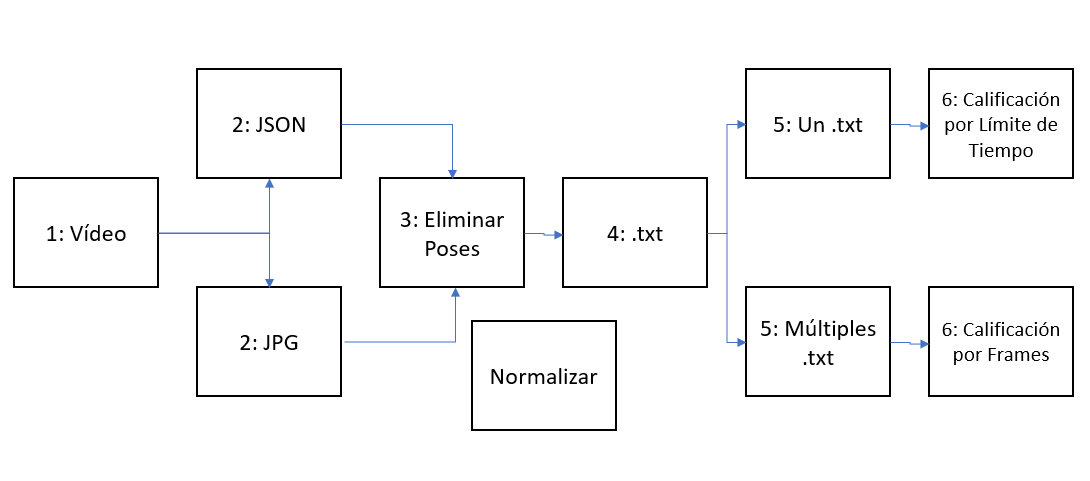
\includegraphics[width=16cm,height=7cm,]{./Images/pasosaseguir.png}
	\caption{Pasos a Seguir Para la Creación de Mapas}
	\footnotesize Fuente: Elaboración Propia
	\label{pasosaseguir}
\end{figure}




\subsubsection{Conversión de Vídeo a JSON y JPG}

El primer paso es la conversión de un vídeo grabado para la creación de un mapa y emplear un Script para ejecutar la Demo,
\subsubsection{Conversión de JSON a .txt}
\subsubsection{Eliminación de Poses}



 y la decisión sobre como disminuir la cantidad de poses y eliminar las poses restantes, para solo tener las poses clave con las cuales comparar.

\subsection{Comparación entre dos Poses}

Esta es considerada la tarea más compleja y laboriosa de elaborar, ya que requiere del estudio previo del modelo BODY\_25 selecto, manejo de los Scripts en C Sharp, estudio relacionado a Point Set Registration y Point Cloud. 


\subsubsection{Visualizar Movimientos del Usuario y Poses a Imitar}

La idea original consta de tres partes, observar desde el Output de la cámara al usuario y sus movimientos y mostrar al costado un vídeo cualquiera para copiar los movimientos, al estar apagada la cámara se verá en azul, como se nota en la figura \ref{primerintento}.  Se realizan modificaciones de GUI para lograrlo, este no será el producto final, es más dirigido a la facilidad de pruebas, para observar los movimientos del usuario del lado izquierdo y el vídeo a imitar del lado derecho.


\subsubsection{Normalización de Puntos Clave/Point Set Registration}

\subsubsection{Exhibir la Precisión de la Comparación al Usuario}

\subsection{Control de Tiempo del Mapa}

\subsubsection{Limite de Tiempo para realizar la posición}

Se la califica y se debe proceder a la siguiente pose cuando el tiempo termine y así se mueva al nuevo tiempo limite de la nueva posición

\subsubsection{Tiempo de Duración del Mapa}



\section{Conversión de un Vídeo a un Mapa}

\subsubsection{Conversión de formato JSON a archivo .txt}

\subsubsection{Eliminación de Archivos .txt}

\subsubsection{Adición del límite de tiempo a las poses}


\section{Diseño De GUI}

